%!TEX root = main.tex

\chapter{Methods for lateral dynamics assessment}

Several analysing methods for vertical dynamics of railway bridges were briefed in \citet[A6.2]{UIC776-2}. Methods that can be applied also on lateral direction are selected:

\begin{quote}

\emph{...}

\emph{Various programs such as ANSYS, NASTRAN, ABAQUS, SAP, FASTRUDL and so on, can be used to obtain the modal responses of bridge decks. Modeling can be done with beam models using torsional characteristics if the bridge is not a skew bridge and the structure is not a special case (see above). However, spatial modeling is necessary in such cases.}
\emph{...}

\end{quote}


\section{Numerical methods}

When the analysis uses numerical methods to directly integrate the dynamic equation, the loads become the dynamic system in the case of vehicles and their internal behavior impacts the response from the structure.

- the two systems can be considered separate systems,

- the vehicle can be considered a finite element.

This last method takes track profile defects into account and deduces the force of interaction between the structure and the vehicle as well as the internal forces in the dynamic system that is built.

In this method, the equation of the dynamics is solved, with or without prior transformation, by using the conventional algorithms for numerical resolution of second-degree differential equations. These numerical methods calculates the response to regularly spaced time intervals(in general). The selected time pitch determines the accuracy of the results and has a bearing on the length of computer calculations.

Numerical integration methods are all based on the search for balanced solutions of the dynamic equation at regular time intervals.

\paragraph{VAMPIRE}

VAMPIRE is a FEM simulation software developed by DeltaRail. It allows the user to build a dynamic model of any rail vehicle and study the response of the vehicle to real measured track geometry or user specified inputs in the form of track displacements and external force inputs. Rail vehicles can be modeled with simulated instrumentation allowing almost any aspect of behavior to be studied. 

\begin{figure}[h!]
    \centering
    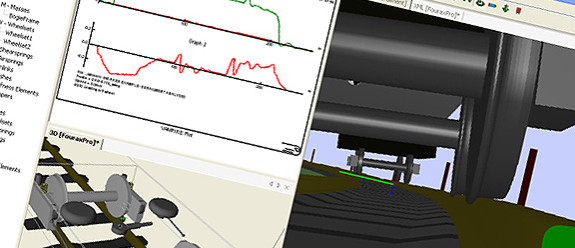
\includegraphics[width=0.8\textwidth]{vampire}
    \caption{A sample project being conducted in VAMPIRE}
    \label{fig:vampire}
\end{figure}

There are also many similar simulation software on the market which puts emphasis on railway vehicle dynamic behavior, but VAMPIRE is specially selected for introduction because it was the software used by UIC committee, whose report series originally proposed 1.2Hz criterion by using the assistance of VAMPIRE. Also, the output results provided by UIC reports is an important foundation for the development of new practical method.